\subsection{Architecture de communication hybride \og orientée 
événements\fg{}}
\label{sec:comm_event}

Cette architecture est une combinaison des contributions présentées dans 
\cite{Desprat2016,Desprat2017} : elle repose sur les éléments du 
framework orienté événements (Section \todo{ref modele event}) qui sont également 
en relation avec la couche réseau (Figure \ref{fig:archievent}).
\begin{figure}[ht]
	\centering
	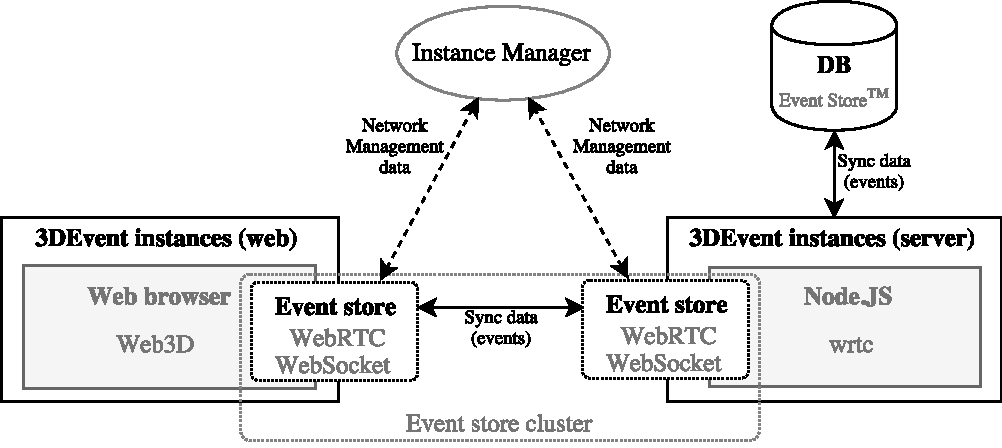
\includegraphics[width=\columnwidth]{eps/archi.pdf}
	\caption{Architecture de communication \og orientée événements\fg{}}
	\label{fig:archievent}
\end{figure}

\subsubsection{Spécificité des composants de l'architecture}
L'Event Store est un composant clé dans le traitement des événements. Présent 
sur chaque pair, il prend en entrée des événements de deux natures : ceux qu'il a 
générés via la partie commande (internes) et ceux reçus via le réseau 
principalement (externes). 
L'Event Store produit en sortie des événements dits \og 
cohérents\fg{} qui peuvent être publiés par la suite sur l'Event Publisher.
Un Event Store est composé de deux types d'éléments : 
\begin{itemize}
	\item l'\gls{ESM} qui gère les flux d'événements : structure de données 
	présente dans chaque Event Store qui doit permettre l'accès en lecture et en 
	écriture des agrégats qu'elle contient. 
	Un \gls{ESM} contient des flux d'événements ordonnés temporellement 
	pour chaque agrégat géré ;
	\item les \glspl{NB} qui servent de connecteurs réseaux : responsables de la 
	gestion d'une connexion \gls{P2P}, i.e. gère le flux de données entrant et 
	sortant vers chaque pair auquel ils sont reliés.
\end{itemize}

La Figure \ref{fig:archievent} montre des pairs (appelés instances) de différentes 
natures :
\begin{itemize}
	\item Instance Web :  produit, stocke et relaie des événements aux autres 
	instances.
	\item Instance Serveur : stocke et relaie des événements aux autres instances 
	et à la base de données. 
\end{itemize}

En plus de servir de relais comme une Instance Serveur, une Instance Web est 
productrice d'événements. C'est en général le type d'instance par lequel un 
utilisateur accédera à l'application. Les Instances Serveurs, en comparaison avec 
l'architecture présentée précédemment, sont des \og serveurs\fg{} qui participent 
directement à la couche réseau. En cela, ils aident à la dissémination des données 
et peuvent rapidement être montés pour garantir une disponibilité des données 
auprès des autres instances (notamment en cas de panne).
Toutes les instances sont coordonnées par l'\gls{IM} qui est responsable de mettre 
les pairs en relation. Il est notamment le serveur responsable dans le mécanisme 
de \textit{signalling}. 

L'ensemble des Event Stores forme une grappe (\textit{cluster}) qui gère le 
journal d'événements partagé de manière répartie entre toutes les instances.
\subsubsection{Gestion du stockage}
\paragraph{Local avec l'\gls{ESM}}
Lorsque l'Event Store reçoit de nouveaux événements, l'\gls{ESM} crée ou 
récupère le flux d'événements associé à l'agrégat dans un premier temps. Puis, il 
stocke l'événement à la suite de ceux présents dans le flux de l'agrégat.

\paragraph{Long-terme et distant avec une base de données fonctionnelle}
Dans un contexte industriel de collaboration, l'information doit être disponible sur le 
long-terme, facilement accessible par l'entreprise. La persistance à 
long-terme stocke le journal d'événements qui est la 
source de vérité de l'application. Elle peut également stocker des projections 
prédéfinies, calculées à la volée ou encore des \textit{snapshots} de l'application.

Sur la base du modèle orienté événements, les données à stocker sont les 
événements. Ils sont immuables et 
constituent des données purement fonctionnelles\todo{voir section \gls{ES} vs CS}.
L'utilisation d'une base de données fonctionnelle permet de se reposer sur 
l'immuabilité des événements.
L'argument souvent opposé à l'utilisation de telles bases est le coût de l'espace de 
stockage. Or le coût de la redondance et de la non localité du traitement des 
données, a chuté au cours de ces dernières années. 
Une base de données dont les données muent -- i.e où chaque donnée peut être 
modifiée à n'importe quel moment -- ne permet pas de conserver l'historique des 
modifications (ex : \textit{Active Record}). Dans une base de données dite 
fonctionnelle, les données stockées sont immuables -- i.e. elles ne peuventt être modifiée \textit{a posteriori} et fait seulement référence à 
d'autres données immuables. Une telle base de données est \og \textit{une interface vers 
des \textit{snapshots} versionnés}\fg{} \cite{Meric2012}.

Dans le cas de l'\gls{ES}, les événements sont considérés comme des deltas 
(avec quelques métadonnées supplémentaires) sur les agrégats. C'est donc sous 
leur forme originale qu'ils sont stockés. Cela évite également les transformations 
de données (et la perte d'information ou l'ajout de complexité) qui sont nécessaires 
dans les \glspl{ORM}, en lecture et en écriture.

\subsubsection{Gestion de la synchronisation et de la cohérence}
Dans \cite{Desprat2017} lorsqu'un pair initialise ou rejoint la séquence pour 
rejoindre une session collaborative, il évolue pour se synchroniser et intégrer les 
nouveaux événements à son journal.
La Figure \ref{fig:connexionpairs} représente la séquence d'actions nécessaire à 
une instance 3DEvent ($idA$) pour rejoindre le réseau contenant déjà d'autres 
instances 3DEvent. L'action \textit{join} est exécutée lorsqu'un utilisateur envoie 
ses informations de connexion sur un portail de connexion (à partir d'une instance 
web) ou lorsqu'une instance serveur est lancée. Cette action ajoute le nouveau 
pair à la liste des pairs présents sur le réseau. Cette liste est gérée par le 
gestionnaire d'instance, qui la retourne au pair pour lui indiquer les pairs 
avec lesquels il doit se connecter.
Pour chaque pair $idB$ de la liste retournée $ids$, $idA$ utilise le mécanisme de 
signalisation (offre/demande). Le mécanisme est déclenché par l'instanciation d'un 
\gls{NB} dans l'Event Store de $idA$ puis celui de $idB$. Afin de resynchroniser 
les deux pairs (après cette série d'échanges asynchrones), $idA$ et $idB$ 
s'échangent des méta-données sur la situation respective de leurs \gls{ESM} 
afin de se synchroniser\todo{(see refernece sync mechanism}.

\begin{figure}[h]
	\noindent
	\centering
	\includegraphics[width=\columnwidth]{connection.eps}
	\caption{Protocole de connexion au réseau d'instance 3DEvent}
	\label{fig:connexionpairs}
\end{figure}

\paragraph{Cohérence d'un agrégat}
Les événements sont considérés comme \og cohérents\fg{}  lorsqu'il n'y a pas 
d'erreur de cohérence dans l'agrégat, i.e. lorsqu'il n'y a pas de doublon dans les 
numéros de versions et qu'ils sont bien ordonnés. Lorsqu'un \gls{ESM} ne 
rencontre pas de problème de cohérence, alors le 
dernier index correspond au numéro de version de l'agrégat. 

Lorsque l'Event Store reçoit un événement interne, l'\gls{ESM} récupère (ou crée) 
le flux d'événements associés à l'agrégat référencé par l'événement. 
La cohérence de la version est alors vérifiée en comparant la version attendue 
(exposée dans les méta-données de l'événement) et la version actuelle de 
l'agrégat. 
Si les deux numéros de version sont identiques, l'événement est ajouté à la fin du 
tableau du flux pour être stocké dans l'\gls{ESM}, sinon une exception est levée. 
La gestion des exceptions est expliquée dans\todo{détails exception}. 

\paragraph{Mécanisme de gestion de version}
3DEvent intègre une procédure de gestion de version dans l'\gls{EventStore} afin 
de gérer au mieux la cohérence des données (voir Section \todo{ref section}). 
Pour être cohérent, l'agrégat concerné par ces 
événements doit produire une nouvelle version, sans être en conflit avec la 
précédente. En passant la version attendue $v_a$ au gestionnaire de conflits, on 
est à même de la comparer avec la version courante $v_c$. Il existe deux cas où 
un conflit est levé~: 
\begin{enumerate}[label=\alph*)]
	\item \label{i:vi} La version $v_a$ correspond à la valeur d'initialisation
	\item \label{i:vdiff} La version $v_a$ est différente de la version $v_c$
\end{enumerate}
Dans \ref{i:vi}, après une action, la version initiale de l'agrégat ne 
peut être la même. Cet item peut sembler évident mais il est important de le noter 
car il dépend entièrement de la valeur initiale choisie pour les agrégats du 
\gls{framework} (on peut commencer à n'importe quelle valeur -- -1, 0\ldots).
\todo{parler de b), et redite par rapport a au dessus}



\subsubsection{Topologie et Protocole d'échange}
L'architecture hybride orientée \og événements\fg{} tire profit de la présence des 
Instances Serveur pour réduire la responsabilité des pairs producteurs (Instances 
Web) dans la distribution des données. En effet, les Instances Serveur qui 
participent au réseau permettent de proposer plus de points de distribution de 
données directement reliés à la base de données. De ce fait, la politique de 
connectivité entre les pairs peut être réduite, le réseau a une topologie maillée 
partiellement (\textit{partial mesh topology}). 


\subsubsection{Gestion de la cohérence}



Pour chaque événement sauvegarder, l’Event Store publie (push) l’événement sur 
le bus (Event Publisher). Cette mécanique est expliquée dans l'algorithme 
\ref{algo:saveEvent}. \todo{finir explications}

\begin{algorithm} % enter the algorithm environment
	\caption{Sauvegarde d'événements d'un agrégat dans l'Event Store} % 
	%give the algorithm a caption
	\label{algo:saveEvent} % and a label for \ref{} commands later in the document
	\begin{algorithmic} % enter the algorithmic environment
		\Require aggregateId : string, uncommitedEvents : eventMsg[ ], 
		version : number
		%\Ensure $y = x^n$
		\State $expectedVersion \Leftarrow version$
		\For{$eventMsg $ \textbf{in} $uncommitedEvents$}	
		\State{$newMsg \Leftarrow \{type : eventMsg.typeEvt, data : eventMsg, 
			streamId : aggregateId\}$}
		\State{$publish(aggregateId, newMsg, expectedVersion++)$}
		\EndFor
	\end{algorithmic}
\end{algorithm}
\todo{parler de cet algo}
\begin{algorithm} % enter the algorithm environment
	\caption{Ajout d'un événement dans l'Event Store} % 
	%give the algorithm a caption
	\label{algo:addevent} % and a label for \ref{} commands later in the document
	\begin{algorithmic} % enter the algorithmic environment
		\Require streamId: string, event: EventStoreEvent, version: number
		\Ensure event
		\State $stream \Leftarrow streams.getOrCreate(streamId);$
		\If{$ stream.has(version)$}
		\State $throwExceptionVersion(stream,version)$
		\EndIf
		\State $stream.data.set(version,event) $
	\end{algorithmic}
\end{algorithm}

\todo{categories: type d’agregat
	c’est un flux liés a une categorie (exemple geometries) tous les events liés à la 
	categorie.}

\todo{metadata phase sync permet a un nouveau noeud de recup toutes les info 
	manquantes et de les demander de maniere repartie a tous les noeuds}



\begin{algorithm} % enter the algorithm environment
	\caption{Synchronisation d'un n\oe ud de l'Event Store partagé} % 
	%give the algorithm a caption
	\label{algo:synchnode} % and a label for \ref{} commands later in the document
	\begin{algorithmic} % enter the algorithmic environment
		\Require $node : ClusterNode$
		\Ensure $nodeState == synchronized$
		\State $nodeMetadata \Leftarrow node.getMetadata()$
		\If{$nodeMetadata != \{\} $}
		\State $streamsToSync \Leftarrow metadata.getDiff(nodeMetadata)$
		\While{$streamsToSync > 0$}
		\State $streamToSync \Leftarrow streamsToSync.pop()$
		\State $events \Leftarrow  node.getEvents(streamToSync)$
		\If{$! streamToSync.has(version)$}
		\For {$event$ \textbf{in} $events$}
		\State $processEvent(event.streamName, event, 
		event.version)$
		\EndFor 
		\EndIf
		\State $streamsToSync \Leftarrow metadata.getDiff(nodeMetadata)$
		\EndWhile
		\EndIf
		\State $node.endSync()$
	\end{algorithmic}
\end{algorithm}

L'algorithme \ref{algo:synchnode} décrit la synchronisation d'un n\oe ud avec un 
autre n\oe ud dans l'Event Store partagé. Le n\oe ud courant demande le 
différentiel (\textit{diff}) entre ses flux et ceux du n\oe ud $node$ pour 
connaître quels sont les flux à synchroniser. Si un n\oe ud possède les données 
demandées il les envoie. Si le n\oe ud courant reçoit à nouveau les mêmes 
données, elles sont ignorées par le système.






\subsubsection{Discussion des problématiques liées à une architecture de 
communication orientée \og événements\fg{}}
Architecture réactive à l'attrition. Tous les éléments qui participent à la gestion de 
données, actifs dans la distribution ou producteurs de données, sont au même 
niveau. Le réseau \gls{P2P} est renforcé par la présence de pairs destinés à 
faire le relais dans la distribution des données. 

La gestion de la cohérence \todo{finir}


%
%\subsubsection{Gestion de la cohérence}
%
%
%\subsubsection{Respect de la causalité}
%\subsubsection{Convergence des répliques}
%\subsubsection{Préservation de l'intention}

%\paragraph{Connexion des pairs en début de session}




